% https://www.mathematik.uni-marburg.de/~thormae/lectures/graphics1/graphics_4_1_eng_web.html#1
\frame{
\frametitle{OpenGL}
\begin{itemize}
\item OpenGL significa Open Graphics Library, un estándar para la progamación de gráfica.
\item Los comandos de gráficos son implementados por el controlador de la tarjeta gráfica y, por lo tanto, son independientes del hardware de la tarjeta gráfica, del sistema operativo y del administrador de ventanas empleado.
\item Los comandos de gráficos están razonablemente cercanos al hardware y son suficientes para lograr la funcionalidad principal
\item Varias bibliotecas y frameworks se basan en OpenGL y permiten la programación a un mayor nivel de abstracción.
\end{itemize}
}

\frame{
\frametitle{OpenGL Versions}
\begin{itemize}
\item Desde su introducción (1992) OpenGL se ha ampliado continuamente para admitir nuevas funciones de tarjetas gráficas.
\item OpenGL 1.0 (1992), OpenGL 1.1 (1997), OpenGL 1.2 (1998), OpenGL 1.3 (2001), OpenGL 1.4 (2002), OpenGL 1.5 (2003)
\item OpenGL 2.0 (2004), OpenGL 2.1 (2006)
\item OpenGL 3.0 (2008), OpenGL 3.1 (2009), OpenGL 3.2 (2009), OpenGL 3.3 (2010)
\item OpenGL 4.0 (2010), OpenGL 4.1 (2010), OpenGL 4.2 (2011), OpenGL 4.3 (2012), OpenGL 4.4 (2013), OpenGL 4.5 (2014), OpenGL 4.6 (2017)
%\item En esta ponencia, se combina la versi
\item A partir de la  versión 3.1, el Pipeline de funciones fijo ya no esta soportado, por locual es necesario implementar shaders, lo cual dificulta el aprendizaje.
\end{itemize}
}


\frame{
\frametitle{OpenGL ES y WebGL}
\begin{itemize}
\item OpenGL ES (Embedded System) es una versión de OpenGL con funcionalidad reducida para teléfonos móviles, televisores, tabletas, etc.
\item OpenGL ES 1.0 (2003): similar a OpenGL 1.3 (Pipeline Fijo)
\item OpenGL ES 1.1 (2004): similar a OpenGL 1.5 (compatible con versiones anteriores)
\item OpenGL ES 2.0 (2007): similar a OpenGL 2.0 (no compatible con versiones anteriores)
\item OpenGL ES 3.0 (2012): similar a OpenGL 3.3 
\item OpenGL ES 3.1 (2014): similar a OpenGL 4.3
\item OpenGL ES 3.2 (2015): similar a OpenGL 4.3
\item OpenGL ES 3.3 (2017): similar a OpenGL 4.6
%\item OpenGL ES se utiliza para la salida de gráficos asistidos por hardware en muchos teléfonos inteligentes (por ejemplo, iPhone de Apple y dispositivos basados en Android)
\item WebGL esta basado en OpenGL ES 2.0 (y WebGL 2.0 en OpenGL ES 3.0) y permite gráficos 3D en páginas web (compatible con la mayoría de navegadores)
\end{itemize}
}


	
\begin{frame}{OpenGL Shading Language}
\begin{itemize}
\item Las aplicaciones móviles son ejecutadas principalmente en el CPU y la memoria principal
\item Para procesamiento de gráficos, los programas son ejecutados en el GPU el cual tiene su propia memoria local (memoria gráfica).
\item Los programas del GPU son escritos en un lenguaje llamado Shading Language (Lenguaje de sombreado). 
\item La mayoría de los GPUs adoptaron el lenguaje de OpenGL shading Language (OGSL)
\end{itemize}
\end{frame}


\begin{frame}{OpenGL Pipeline (2)}
    \begin{center}
    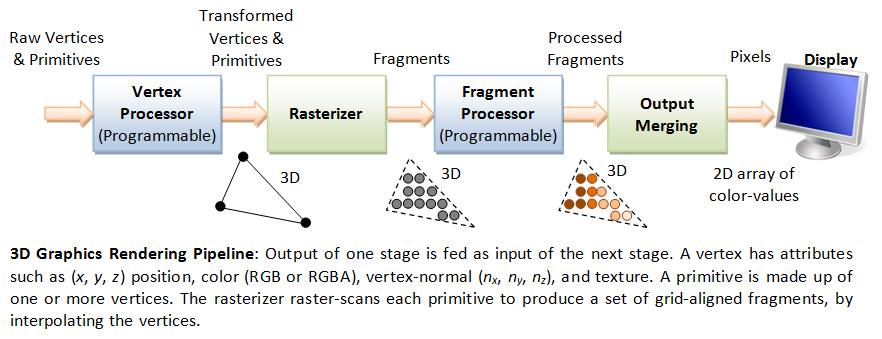
\includegraphics[width=\textwidth]{Figs/Graphics3D_Pipe}
    \end{center}
\end{frame}


\begin{frame}{OpenGL Pipeline (3)}
    \begin{center}
    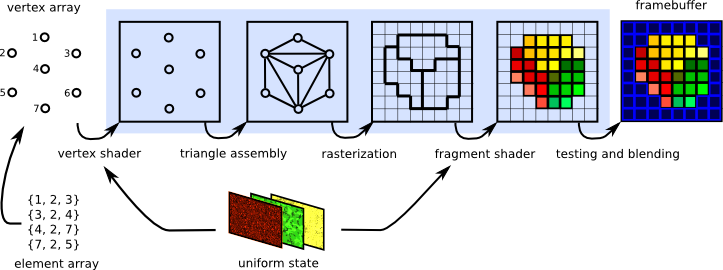
\includegraphics[width=\textwidth]{Figs/evasgl-graphics-pipeline}
    \end{center}
\end{frame}

